\documentclass[aspectratio=169]{beamer}

\usepackage[english]{babel}
\usepackage[utf8x]{inputenc}			
\usepackage{listings}
\usepackage{xcolor}
\usepackage{tikz}
\usetikzlibrary{trees}  % 用於樹狀圖
\lstset{
    language=R,
    basicstyle=\ttfamily\small,
    backgroundcolor=\color{gray!10},
    frame=single,
    breaklines=true,
    showstringspaces=false,
    keywordstyle=\color{blue},
    commentstyle=\color{green!50!black},
    stringstyle=\color{red},
    numbers=none,
    xleftmargin=10pt,
    xrightmargin=10pt,
    framexleftmargin=5pt,
    framexrightmargin=5pt
}

\mode<presentation>						
{
  \usetheme{default}					
  \usecolortheme{default} 			
  \usefonttheme{default}  				
  \setbeamertemplate{caption}[numbered]	
}

\usepackage{graphicx}					
\usepackage{booktabs}					
\usepackage{hyperref}					
\usepackage{subcaption}  
\usepackage{multicol}
\usepackage{hyperref}

\title{Hypothesis Testing}	
\author{Rex Shao-Yu Wang}								
\institute{Department of Agronomy, National Taiwan University}				
\date{May 4, 2026}								

\begin{document}

% Title page
\begin{frame}
  \titlepage
\end{frame}

% Outline
\begin{frame}{Outline}
  \tableofcontents
\end{frame}


\section{Recap}
\begin{frame}{Procedure for Hypothesis Testing}
\begin{enumerate}
    \item State your null and alternate hypothesis
    \item Define significant level $\alpha$
    \item Decide the test statistic ($Z, T,F $)
    \item Find the rejection region (RR)
    \item Calculate your test statistic and compare with RR
    \item Make a decision whether reject $H_0$ or not
\end{enumerate}
\end{frame}



\begin{frame}[label=dTree]{Types of Hypothesis Testing}
    
\footnotesize 
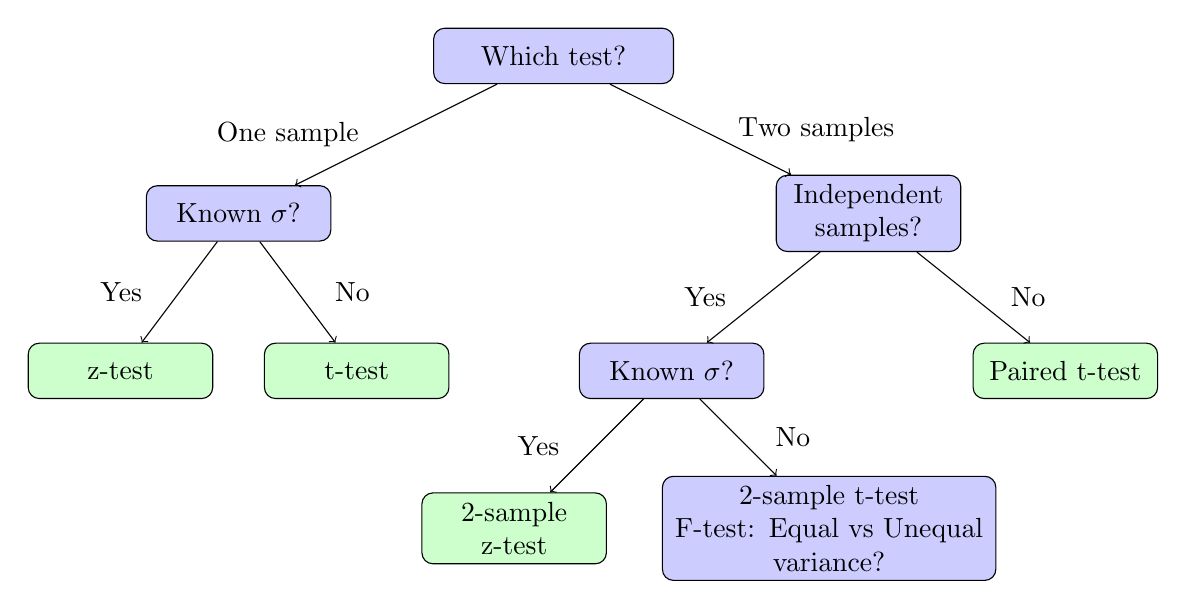
\begin{tikzpicture}[grow=down,level distance=2cm,sibling distance=5cm]
    \tikzstyle{decision} = [rectangle, draw, fill=blue!20, text width=6em, text centered, rounded corners, minimum height=2em]
    \tikzstyle{leaf} = [rectangle, draw, fill=green!20, text width=6em, text centered, rounded corners, minimum height=2em]
    \tikzstyle{edge from parent}=[->, draw]
    \node [decision, text width=8em] (T){Which test?}[sibling distance=8cm] 
    child { node [decision] (S1) {Known $\sigma$?} [sibling distance=3cm] 
        child { node [leaf] {z-test} 
            edge from parent 
            node [left=1em] {Yes} 
        }
        child { node [leaf] {t-test} 
            edge from parent 
            node [right=1em] {No} 
        }
    }
    child { node [decision] (Ind) {Independent samples?} [sibling distance=5cm] 
           child { node [decision] (S2) {Known $\sigma$?}[sibling distance=4cm] 
                child { node [leaf] {2-sample z-test}
                    edge from parent 
                    node [left=1em] {Yes} 
                }
                child { node [decision, text width=4cm] {2-sample t-test\\F-test: Equal vs Unequal\\variance?} [level distance=1.5cm]
                    edge from parent 
                    node [right=1em] {No} 
%                    child { node [leaf, level distance=1cm, text width=4cm] {2-sample t-test} }
                }                
%                child { node  {F-test}                     
%                    edge from parent node [right=1em] {No} }
            }
%        child { %node [decision] {No. Paired samples}
            child { node [leaf] {Paired t-test} 
                edge from parent 
                node [right=1em] {No} 
            }
%        }
    };
    \path (T) to node [left=1em] {One sample} (S1);
    \path (T) to node [right=1em] {Two samples} (Ind);
    \path (Ind) to node [left=1em] {Yes} (S2);
%    \draw (T) -- +(0,-1) |-  {aoeu} (S1);
%    \path (T) |- +(1,-1) -- {oeuid} (S2);
\end{tikzpicture}
\large \centering One-tailed vs Two-tailed
\end{frame}

\section{Two sample t-test}
\begin{frame}{Two sample t-test}
\begin{itemize}
    \item Hypothesis: $H_0: \mu_1 = \mu_2$ vs. $H_A: \mu_1 \neq \mu_2$
    \item Test Statistic:
    \begin{itemize}
        \item Equal Variance $\sigma_1^2 = \sigma_2^2 = \sigma^2$
    \[
    T = \frac{\overline{x_1}-\overline{x_2}-0}{\sqrt{\frac{s_{pooled}^2}{n_1}+\frac{s_{pooled}^2}{n_2}}} \overset{H_0}{\sim} t(n_1+n_2-2), \ where\ s_{pooled}^2 = \frac{(n_1-1)s_1^2+(n_2-1)s_2^2}{(n_1+n_2-2)}
    \]
        \item Unequal Variance $\sigma_1 \neq \sigma_2$
    \[
    T = \frac{\overline{x_1}-\overline{x_2}-0}{\sqrt{\frac{s_{1}^2}{n_1}+\frac{s_{2}^2}{n_2}}} \overset{H_0}{\sim} t(df_{Welch}), \ where\ df_{Welch} = \frac{(\frac{s_1^2}{n_1}+\frac{s_2^2}{n_2})^2}{\frac{(\frac{s_1^2}{n_1})^2}{n_1-1}+ \frac{(\frac{s_2^2}{n_2})^2}{n_2-1}}
    \]
        \end{itemize}
    \item Rejection Region:
    \[
    RR = \{\lvert T \rvert \ge t_{\frac{\alpha}{2}}(df)\} = \{T \ge t_{\frac{\alpha}{2}}(df)\ or\ T \le -t_{\frac{\alpha}{2}}(df)\}
    \]
\end{itemize}

\end{frame}

\begin{frame}[fragile]{Two sample t-test}
We get data1 and data2, and we want to test whether $\mu_1 = \mu_2$ under $\alpha=0.05$
\begin{lstlisting}
data1 <- c(27, 24, 18, 29, 30, 27)
data2 <- c(23, 28, 20, 19, 35, 23)
\end{lstlisting}
\begin{itemize}
    \item Equal Variance
\begin{lstlisting}
t.test(data1, data2, mu = 0, var.equal = TRUE, conf.level = 0.95)    
\end{lstlisting}

    \item Unequal Variance
\begin{lstlisting}
t.test(data1, data2, mu = 0, var.equal = FALSE, conf.level = 0.95)    
\end{lstlisting}
\end{itemize}
\end{frame}

\section{F-test}
\begin{frame}{F-test}
\begin{itemize}
    \item Hypothesis: $H_0: \sigma_1^2 = \sigma_2^2$ vs. $H_A: \sigma_1^2 \neq \sigma_2^2$
    \item Test Statistic: the ratio of two sample variances
    \[
    F = \frac{s_1^2}{s_2^2} \overset{H_0}{\sim} F_{n_1-1, n_2-1,[\alpha/2]}
    \]
    \item Rejection Region:
    \[
    RR = \{F > F_{n_1-1, n_2-1,[\alpha/2]}\} 
    \]
\end{itemize}
\end{frame}



\begin{frame}[fragile]{F-test}
Assume we get two sample: group1 and group2\\
We want to test whether the population variance of these two groups are different?\\
\begin{lstlisting}
# Sample data
group1 <- c(15.2, 16.5, 14.8, 16.9, 15.5, 15.8)
group2 <- c(14.0, 13.8, 15.2, 13.9, 14.1, 14.5)

# Perform the F-Test
var.test(group1, group2)
\end{lstlisting}
\end{frame}

\section{Paired t-test}
\begin{frame}{Paired t-test}
\begin{itemize}
    \item The differences between each pair$(i)$ of sample units
    \[
    d_i = x1_i - x2_i
    \]
    \item Calculate $\overline{d}$ and $s_d$
    \item Hypothesis: The population mean of the differences is zero
    \[
    H_0: \mu_d = 0\ \ vs.\ H_A: \mu_d \neq 0
    \]
    \item Test Statistic:
    \[
    t = \frac{\overline{d}-0}{s_d/\sqrt{n}}
    \]
    \item Rejection Region:
    \[
    RR = \{|t| > t_n-1\} 
    \]
\end{itemize}
\end{frame}

\begin{frame}[fragile]{Paired t-test}
We got two groups: group1 and group2.
We knew that these two groups are dependent
\begin{lstlisting}
# Sample data
group1 <- c(rnorm(100, mean = 14, sd = 0.3))
group2 <- c(rnorm(100, mean = 13, sd = 0.2))

# Perform the paired t -test
t.test(group1, group2, paired = TRUE)
\end{lstlisting}
\end{frame}

\section{Lab Report}
\begin{frame}{Lab Report}
\begin{itemize}
    \item The report file will be in the NTU COOL Assignment section
    \item Submit your file in pdf format
    \item Deadline: 5/10 (Sun) 23:59
    \item Late submission is not accepted
\end{itemize}
\end{frame}

\end{document}




